\chapter{Basics}

\section{JavaScript}
There are a few big advantages offered by \textbf{\gls{JS}}. Maybe the biggest advantage is that it comes with the web browser, so everybody can run it by simply typing in an \gls{URL}. This offers great possibilities, since the users don't have to install any software package. The provided application is immediately ready to use once it was loaded. Today \gls{JS} is the most used programming language world wide (Picture: \ref{fig:JS}). \gls{JS} first appeared in 1995, originally developed at Netscape by Brendan Eich it had a simple purpose, dynamically manipulating the HTML DOM in the browser. At the same time a company called Sun worked on a programming language called Java, Netscape and Sun decided to work together. Netscape noticed that it would be good marketing to rename LiveScript to \gls{JS}. Since Java already had a growing community and was liked by many people, so Netscape took the chance and \gls{JS} was born. However both language don't share a lot of things together, Java is a normal, static, and highly typed programming language, it runs on a virtual machine and needs to be compiled, whereas the single threaded \gls{JS} only runs in the browser and is script. Nevertheless they share the C related syntax and some similarities regarding naming conventions, both support object oriented programming.The following analysis shall show why Java Script is in many ways superior for web development. Jeff Attwood the co-founder of the  computer programming question-and-answer website Stack Overflow and Stack Exchange once said "Any application that can be written in \gls{JS}, will eventually be written in JavaScript". \cite{HistoryJS1} \cite{HistoryJS2} \cite{HistoryJS3}

\begin{figure}
	\centering
	\includegraphics[scale=0.5]{bilder/grundlagen/jsUsage.png}
	\caption{Github Repositories sorted after used language} source:\cite{JS}
	\label{fig:JS}
\end{figure}

\newpage

\subsection{JavaScript Distributed Architectures}
Most modern web designs rely on they three-tier architecture. On the server side computing is done and data is stored in databases. The client fetches the data from the server and displays it. Often the user is able to change the data on the client side. 
\begin{figure}[hb]
	\centering
	\includegraphics[scale=0.5]{bilder/grundlagen/Three-Tier.png}
	\caption{Github Repositories sorted after used language} source:\cite{JS}
	\label{fig:JS}
\end{figure}
For example deleting or adding a user, a request is sent to the server and a database change is done. For client side it is mandatory to use \gls{JS}, but on server side  a great spectrum of languages is available, Java, CSharp, PHP, Ruby these are just the most famous one. Once a user is added on client side, code is needed there in JavaScript and same action needs to be implemented in a different language on server, therefore one needs to provide duplicated code. 
But the JavaScript ecosystem is undergoing rapid growth, with Node.js \gls{JS} is coming to the server and developers are now able to do whole applications in \gls{JS}. That's huge step, distributed systems that can use shared modules. It even affects the job market, front-end developers and back-end developers have been two separated jobs for over decades but now are one. People do not need to learn two languages anymore if they want to do full-stack web development, everything is covered with JavaScript.

\begin{figure}
	\centering
	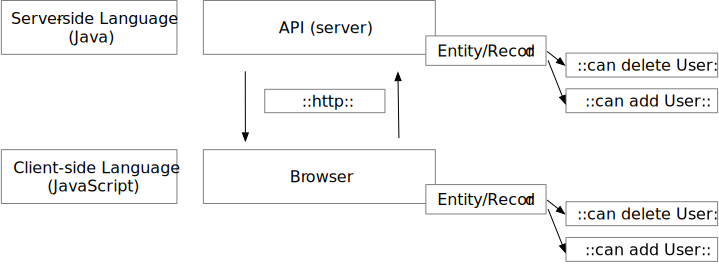
\includegraphics[scale=0.5]{bilder/grundlagen/Entity1.png}
	\caption{Github Repositories sorted after used language} source:\cite{JS}
	\label{fig:JS}
\end{figure}
\begin{figure}
	\centering
	\includegraphics[scale=0.5]{bilder/grundlagen/Entity2.png}
	\caption{Github Repositories sorted after used language} source:\cite{JS}
	\label{fig:JS}
\end{figure}


\subsection{Mutli-Platform Support}

Deploying an application for the web browser is only one aspect of modern web development, often a separate implementation is needed for mobile devices. Two major operating systems are currently dominating the smart-phone market Android and IOS. Both support native App developing but that brings back the problem of having to implement the same functionality twice. Sure smart-phone Apps are different from browser based applications, starting with the touch event and ending up with totally different layouts, but however taking back the adding and deleting a user example from the last section, the main action still stays the same. A user needs to be created and needs be deleted on client side and server side. With JavaScript a developers can take advantage of modern frameworks like React Native or Electron, this topic will be further evaluated in later sections.

\begin{figure}[hb]
	\centering
	\includegraphics[scale=0.3]{bilder/grundlagen/marktanteil.png}
	\caption{Market share operating systems based on sold phones} source:\cite{JS}
	\label{fig:MS}
\end{figure}


\subsection{Scalability}











